\section{Testy rozwiązania}
	\label{final:testy}

	\subsection{Generowanie grafów}
		\label{final:testy:generowanie}

		Istotnym etapem projektu było przygotowywanie danych testowych. Do tego celu został zaimplementowany generator grafów(klasa GraphGenerator). Generowane grafy były zapisywane do pliku w celu ich późniejszego wykorzystania do analizy. Etap generowania grafów był etapem, który zajął najwięcej czasu w procesie testowania i wynosił on kilka dni. Grafy, które zostały wygenerowane zajęły około 10 GB pamięci na dysku.
% \\
% TABELKA
% \\
	\subsection{Przeprowadzone testy}
		\label{final:testy:przyklad1}
		Poniżej zamieszczone są wykresy ilustrujące jak zmieniały się prawdopodobieństwo spójności, średni rozmiar największej składowej spójnej, rozmiar największej składowej spójnej w zależności od liczby wierzchołków oraz promienia. Dla każdego grafu test był powtarzany 100 razy(parametr ---repeats=100)

		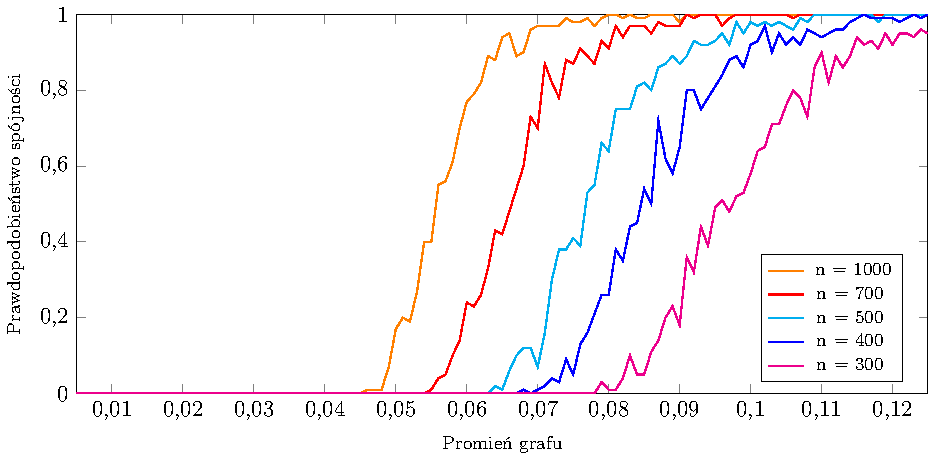
\includepdf[scale=0.9, pages={1}]{500-0_0010_125_consistency_prob.pdf}
		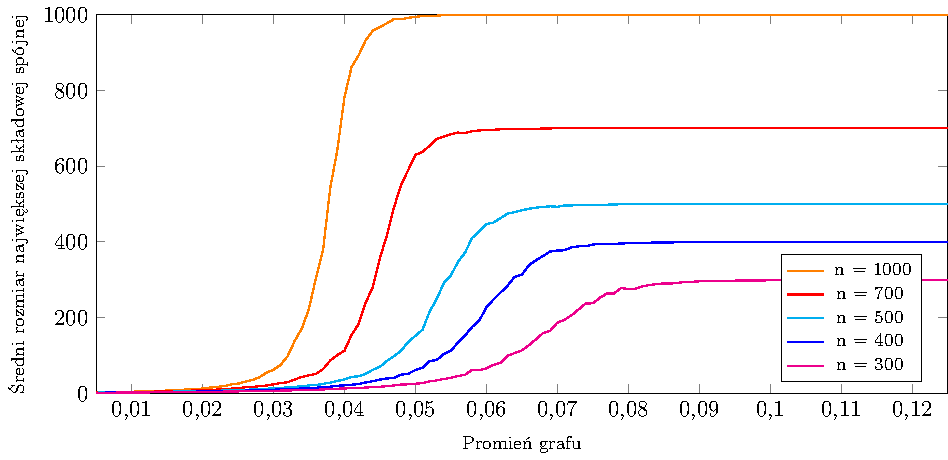
\includepdf[scale=0.9, pages={1}]{500-0_0010_125_max_comps_sizes_means.pdf}
		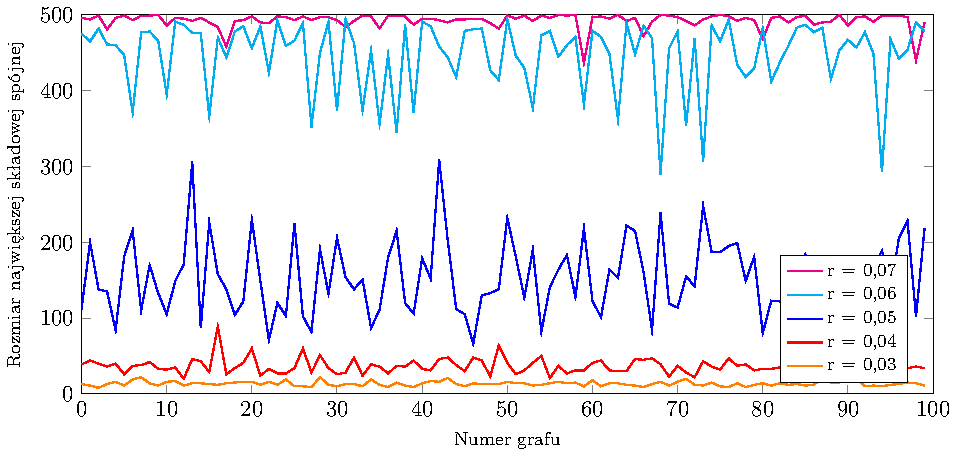
\includepdf[scale=0.9, pages={1}]{500-max_comps_sizes.pdf}
		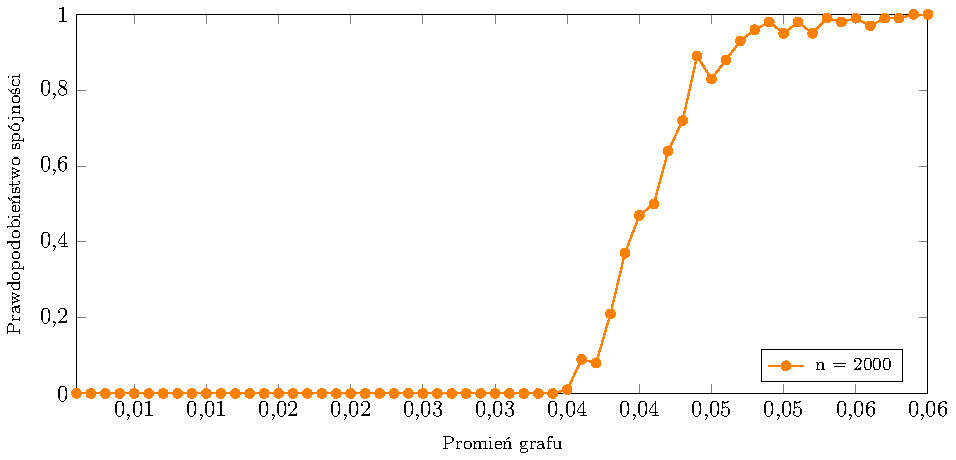
\includepdf[scale=0.9, pages={1}]{2000-0_06_0-consistency_prob.pdf}
		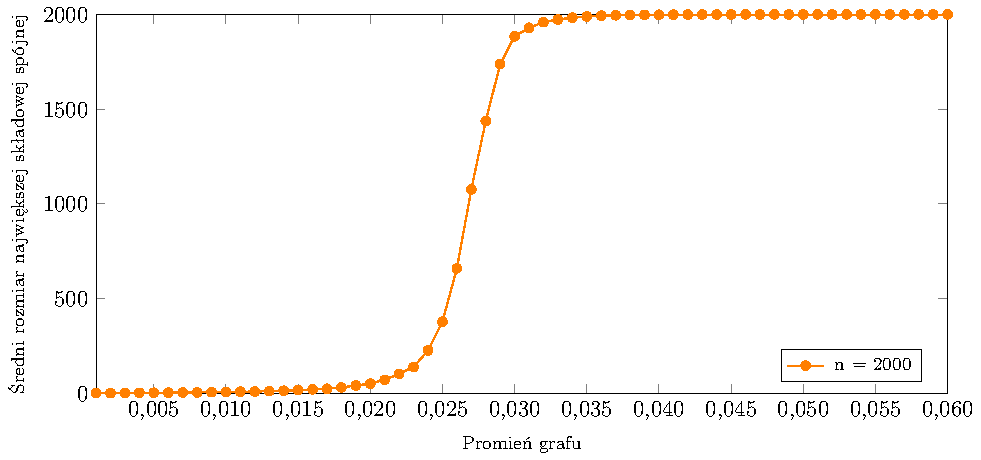
\includepdf[scale=0.9, pages={1}]{2000-0_06_0-max_comps_sizes_means.pdf}
		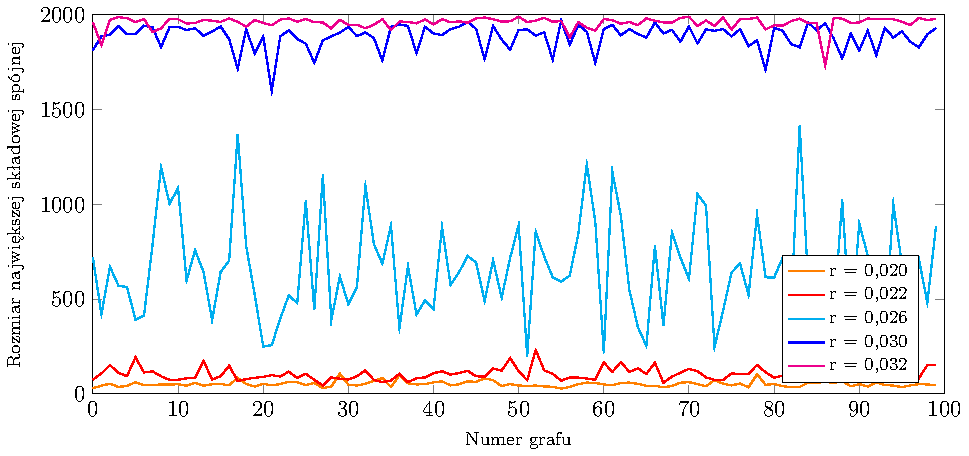
\includepdf[scale=0.9, pages={1}]{2000-max_comps_sizes.pdf}
		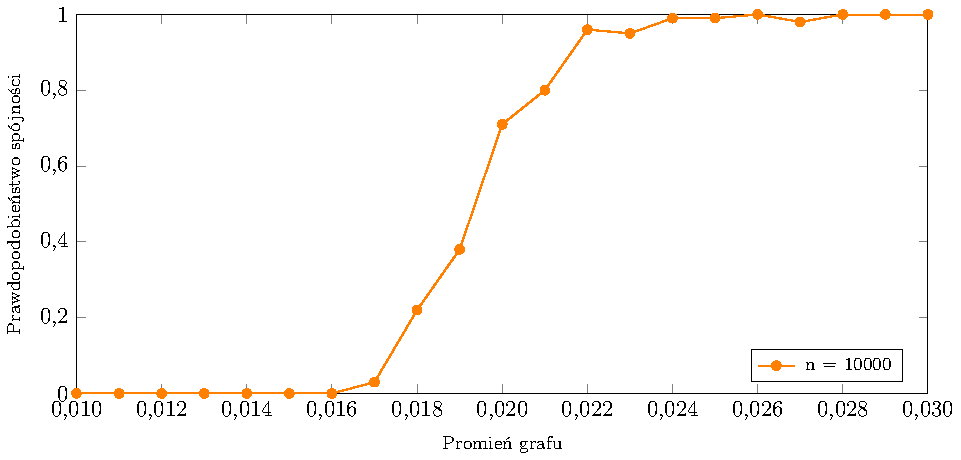
\includepdf[scale=0.9, pages={1}]{10000-0_03_0-consistency_prob.pdf}
		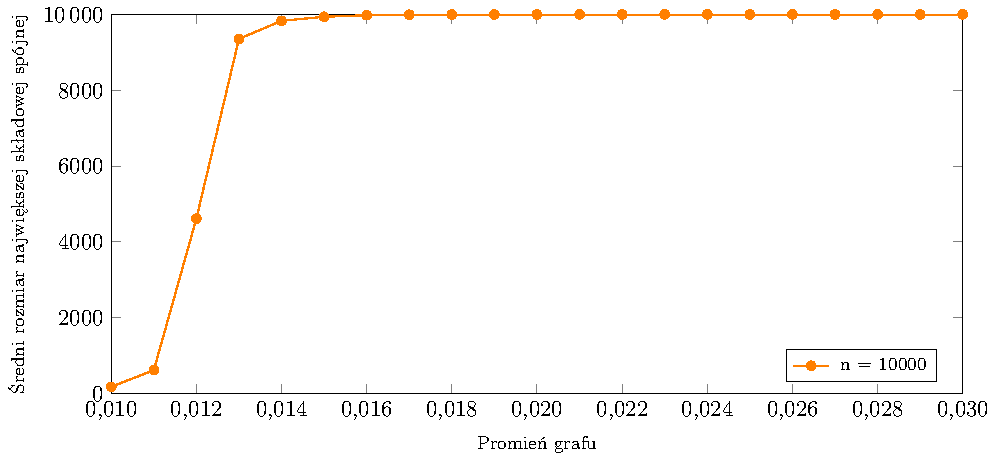
\includepdf[scale=0.9, pages={1}]{10000-0_03_0-max_comps_sizes_means.pdf}
		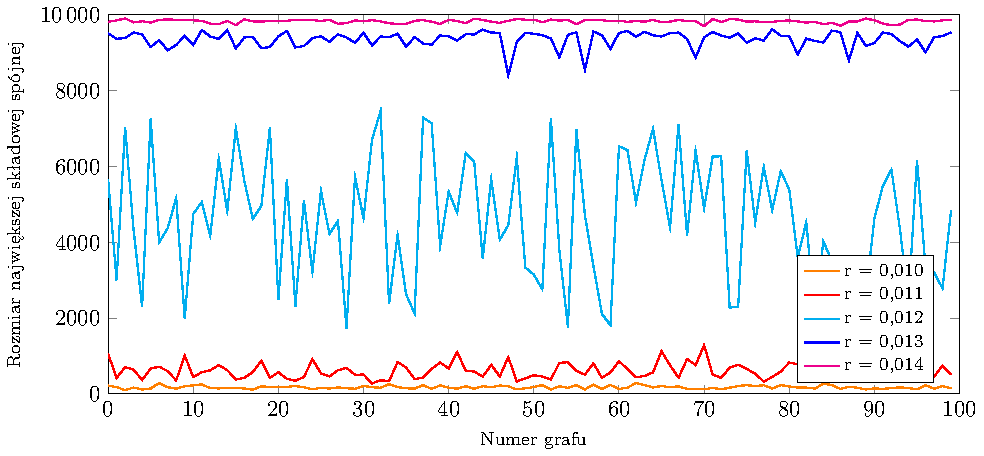
\includepdf[scale=0.9, pages={1}]{10000-max_comps_sizes.pdf}
		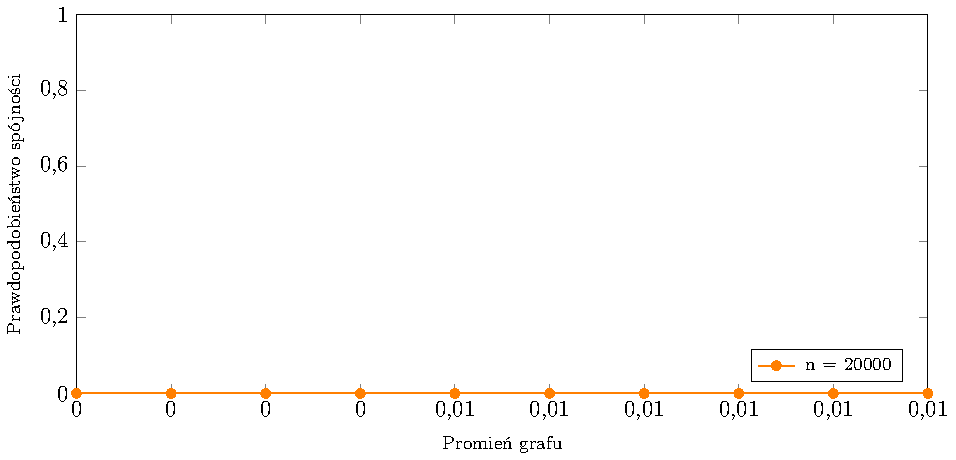
\includepdf[scale=0.9, pages={1}]{20000-0_01_0-consistency_prob.pdf}
		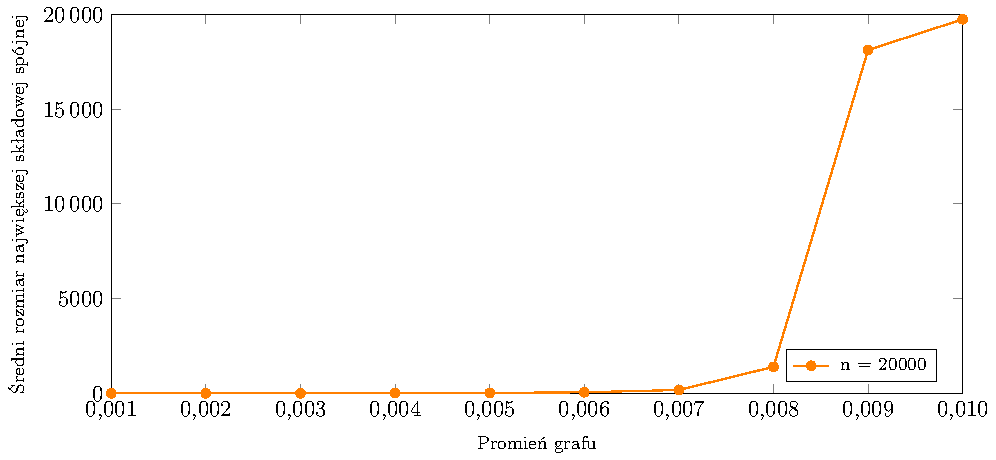
\includepdf[scale=0.9, pages={1}]{20000-0_01_0-max_comps_sizes_means.pdf}
		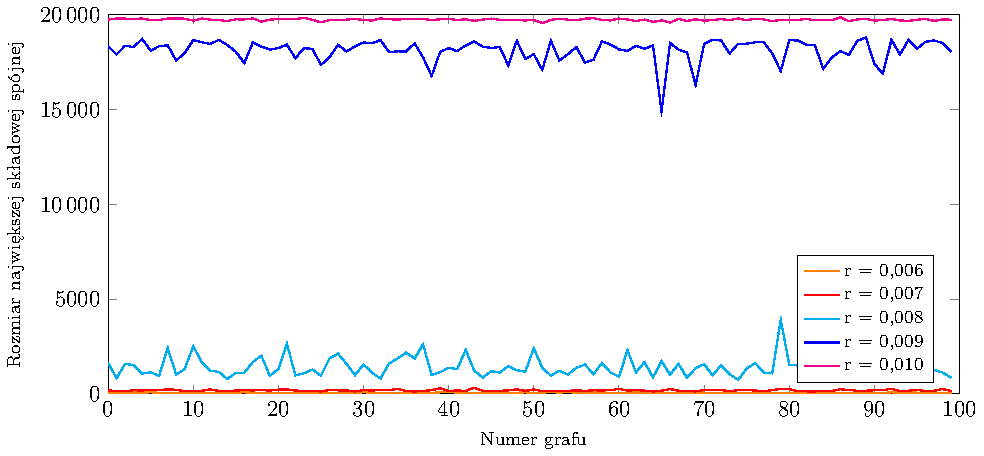
\includepdf[scale=0.9, pages={1}]{20000-max_comps_sizes.pdf}

	\subsection{Wnioski}
		\label{final:testy:wnioski}
	
	Z zamieszczonych rysunków można zauważyć, że wraz że wraz ze wzrostem liczby wierzchołków grafu rośnie również prawdopodobieństo, że będzie on spójny. Podobna zależność występuje przy zmianie promienia. Warto również wspomnieć o tym, że przy małej liczbie wierzchołków oraz małemu promieniowi prawdopodobieństwo spójności jest zerowe. W pewnym momencie następuje nagły wzrost prawdopodobieństa i rośnie ono dosyć szybko. Następnie zwalnia na poziomie 90 procent i powoli dąży do maksymalnej wartości.

	W skrócie z przeprowadzonych testów można wyciągnąć następujące wnioski:
	\begin{itemize}
		\item Wraz ze wzrostem liczby wierzchołków rośnie prawdopodobieństwo spójności sieci
		\item Wraz ze wzrostem promienia rośnie prawdopodobieństwo spójności sieci
		\item Im większa liczba wierzchołków w grafie tym większy średni rozmiar największej składowej spójnej
		\item Im większy promień grafu tym większy średni rozmiar największej składowej spójnej	
	\end{itemize}
